\chapter{Preliminaries}\label{chap:preliminaries}

This chapter contains definitions and concepts related to the study of symmetries and partial symmetries of graphs. We also provide examples to illustrate and explain these concepts. Examining the symmetries and partial symmetries of graphs requires knowledge from different fields of mathematics, such as graph theory, group theory, and semigroup theory.

\section{Graph theory}

In this section, we introduce the basics of graph theory. We examine different ways to represent graphs, what subgraphs and induced subgraphs are, and define graph isomorphism and automorphism.

Firstly, we mention some examples and usages of graphs in real-world applications. For example, we can represent the road network as a graph with crossroads or dead ends acting as imaginary vertices and the roads connecting them as edges. Indeed, graphs are used in video game development to represent the road network.

While the term graph is commonly used formally in mathematics, the graphs appearing in real-world applications are often referred to as networks. Some examples of networks include social networks, used to represent individuals and their relationships, or neural networks, most commonly used in artificial intelligence.

\begin{figure}[H]
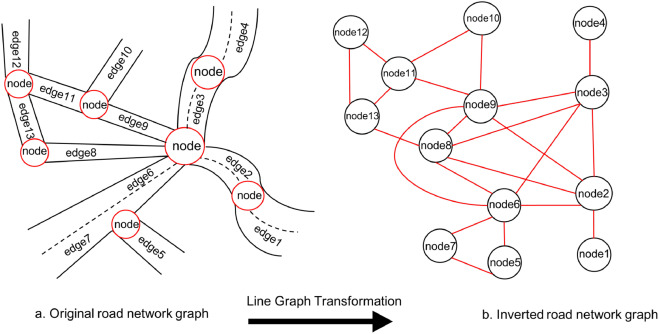
\includegraphics[width=\textwidth,height=\textheight,keepaspectratio]{images/road_graph.jpg}
\caption{Example of a road network represented as a graph \cite{gha21}.}
\label{fig:road_graph}
\end{figure}

The definitions used in this section are taken from the book \cite{Wes01}.

\begin{definition}
\label{def:graph}
A graph $G$ is a triple consisting of a vertex set V(G), an edge set E(G), and a relation that associates with each edge two vertices (not necessarily distinct) called its endpoints.
\end{definition}

Let's examine the graph in Fig. \ref{fig:graph_example}. The vertex set of this graph is $\{a, b, c, d, e\}$ and the edge set is $\{e_1, e_2, e_3, e_4,e_5, e_6, e_7\}$. As we can see in the picture, the edge $e_1$, as well as the edge $e_2$ have the vertices $a$ and $b$ as its endpoints, the edge $e_4$ has vertices $b$ and $c$ as its endpoints, and the edge $e_7$ has the vertex $d$ as both of its endpoints. We also say that an edge is $incident$ to its endpoints. We define the following terms to refer to edges whose endpoints are equal and edges that share the same pair of endpoints:

\begin{figure}[H]
\begin{center}
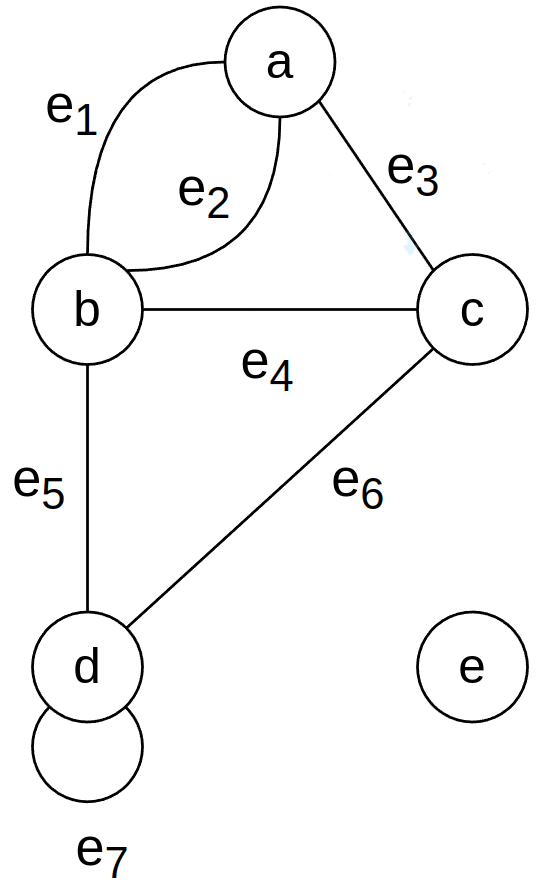
\includegraphics[scale=0.2, keepaspectratio]{images/graph_example.png}
\end{center}
\caption{An example of a graph with five vertices and seven edges.}
\label{fig:graph_example}
\end{figure}

\begin{definition}
\label{def:multiedge_loop}
A loop is an edge whose endpoints are equal. Multiple edges are edges having the same pair of endpoints.
\end{definition}

By examining the definition of the graph from above, we can see that the relation that associates an edge with two vertices (the adjacency relation) is symmetric, and such graphs are called undirected. When the relation between vertices does not need to be symmetric, we talk about directed graphs, which are defined as follows:

\begin{definition}
\label{def:digraph}
A directed graph or digraph G is a triple consisting of a vertex set V(G), an edge set E(G), and a function assigning each edge an ordered pair of vertices. The first vertex of the ordered pair is the tail of the edge, and the second is the head; together, they are the endpoints. We say that an edge is an edge from its tail to its head.
\end{definition}

When visually representing an edge in a digraph, we draw an arrow near the head vertex. We can see an example of an undirected graph and a digraph in Fig. \ref{fig:dir_undir_example}.

\begin{figure}[H]
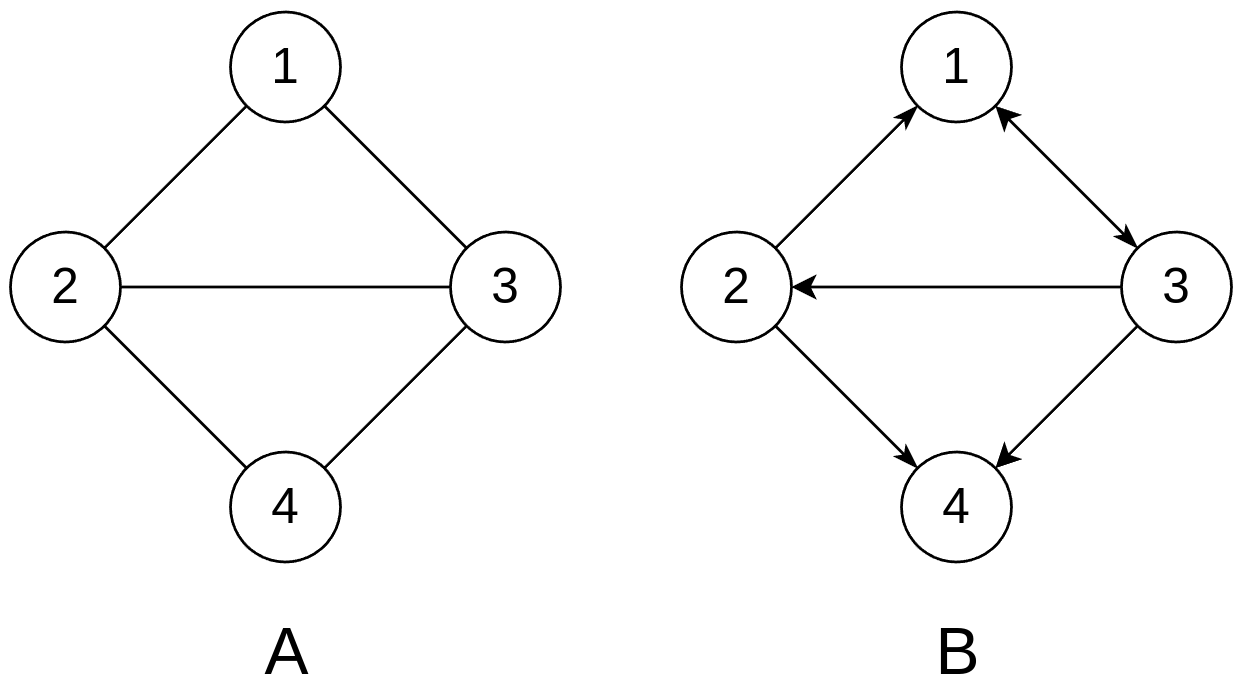
\includegraphics[width=\textwidth,height=\textheight,keepaspectratio]{images/directed_undirected_graph.png}
\caption{An example of an undirected graph (A) and a directed graph (B).}
\label{fig:dir_undir_example}
\end{figure}

\subsection{Finite simple graphs}

In our work, we focus on a class of graphs called finite simple graphs. A finite simple graph is an undirected graph with a finite vertex set that does not allow loops or multiple edges.

\begin{definition}
\label{def:simple_graph}
A simple graph is a graph having no loops or multiple edges. We specify a simple graph by its vertex set and edge set, treating the edge set as a set of unordered pairs of vertices and writing e = uv (or e = vu) for an edge e with endpoints u and v.
\end{definition}

\begin{definition}
The $complement$ $\bar{G}$ of a simple graph $G$ is the simple graph with vertex set $V(G)$ defined by $uv \in E(\bar{G})$ if and only if $uv \notin E(G)$. A clique in a graph is a set of pairwise adjacent vertices. An independent set (or stable set) in a graph is a set of pairwise nonadjacent vertices.
\end{definition}

In total, there are $2^{\frac{n(n-1)}{2}}$ possible undirected simple graphs with $n$ vertices. Each vertex can be connected with an edge to $n-1$ different vertices, and since the graph is undirected, we ignore repetitions, hence $\frac{n(n-1)}{2}$. We then have two choices for each pair of vertices: either they are connected by an edge or not.

From this point on, "graph" refers to a finite simple graph unless specified otherwise.

\begin{definition}
\label{def:degree}
The degree of vertex v in a graph G, written $d_G(v)$ or $d(v)$, is the number of edges incident to v. The maximum degree is $\Delta(G)$, the minimum degree is $\delta(G)$, and G is regular if $\Delta(G) = \delta(G)$.
\end{definition}

The maximum degree of a vertex in graph G on $n$ vertices is $n - 1$. The minimum degree of a vertex is 0, and such vertices are called $isolated$. If G is a complete graph, the minimum and maximum degrees are $n - 1$. In a $k$-regular graph, all vertices are of the same degree $k$.

\subsection{Subgraphs and induced subgraphs}

In this section, we talk about subgraphs and induced subgraphs. We start by listing the definitions of walks, trails, and paths. We then also provide the definitions for subgraphs and components of a graph.

\begin{definition}
\label{def:walk}
A walk is a list $v_0, e_1, v_1, ..., e_k, v_k$ of vertices and edges such that, for $1 \leq i \leq k$, the edge $e_i$ has endpoints $v_{i-1}$ and $v_i$. A trail is a walk with no repeated edge. A u, v-walk or u, v-trail has first vertex u and last vertex v; these are its endpoints. A u, v-path is a path whose vertices of degree 1 (its endpoints) are u and v; the others are internal vertices.

The length of a walk, trail, path, or cycle is its number of edges. A walk or trail is closed if its endpoints are the same.
\end{definition}

\begin{definition}
\label{def:subgraph}
A subgraph of a graph G is a graph H such that V(H) $\subseteq$ V(G) and E(H) $\subseteq$ E(G) and the assignment of endpoints to edges in H is the same as in G. We then write H $\subseteq$ G and say that "G contains H".

A graph G is connected if each pair of vertices in G belong to a path; otherwise, G is disconnected.
\end{definition}

\begin{definition}
The components of a graph $G$ are its maximal connected subgraphs.
\end{definition}

Every connected graph has exactly one component. A disconnected $n$-vertex graph has at least two and at most $n$ components.

Note that in the above definition of subgraph, if $u, v \in V(H)$ and $(u,v) \in E(G)$, then $(u, v)$ does not need to be in $E(H)$. However, we focus on specific types of subgraphs called induced subgraphs.

\begin{definition}
\label{def:induced_subraph}
A cut-edge or cut-vertex of a graph is an edge or vertex whose deletion increases the number of components. We write G - e or G - M for the subgraph of G obtained by deleting an edge e or set of edges M. We write G - v or G - S for the subgraph obtained by deleting a vertex v or set of vertices S. An induced subgraph is a subgraph obtained by deleting a set of vertices, along with their incident edges. We write G[T] for G - $\overline{T}$, where $\overline{T}$ = V(G) - T; this is the subgraph of G induced by T.
\end{definition}

In other words, an induced subgraph $H$ is a subgraph obtained by taking a subset of vertices of graph $G$ and all edges that are incident to these vertices in $G$.

In Fig. \ref{fig:induced_subgraphs}, we have a graph $G$. We obtain an induced subgraph $G[T]$, where $T = \{ 1, 2, 4 \}$, by deleting a set of vertices $V(G) - T$ as well as their incident edges. In particular, we delete the vertex $3$ and its incident edges, so $e_3$ and $e_4$.

A graph with $n$ vertices has at most $\displaystyle \sum_{m=0}^{n}{n \choose m} = 2^n$ induced subgraphs.

\begin{figure}[H]
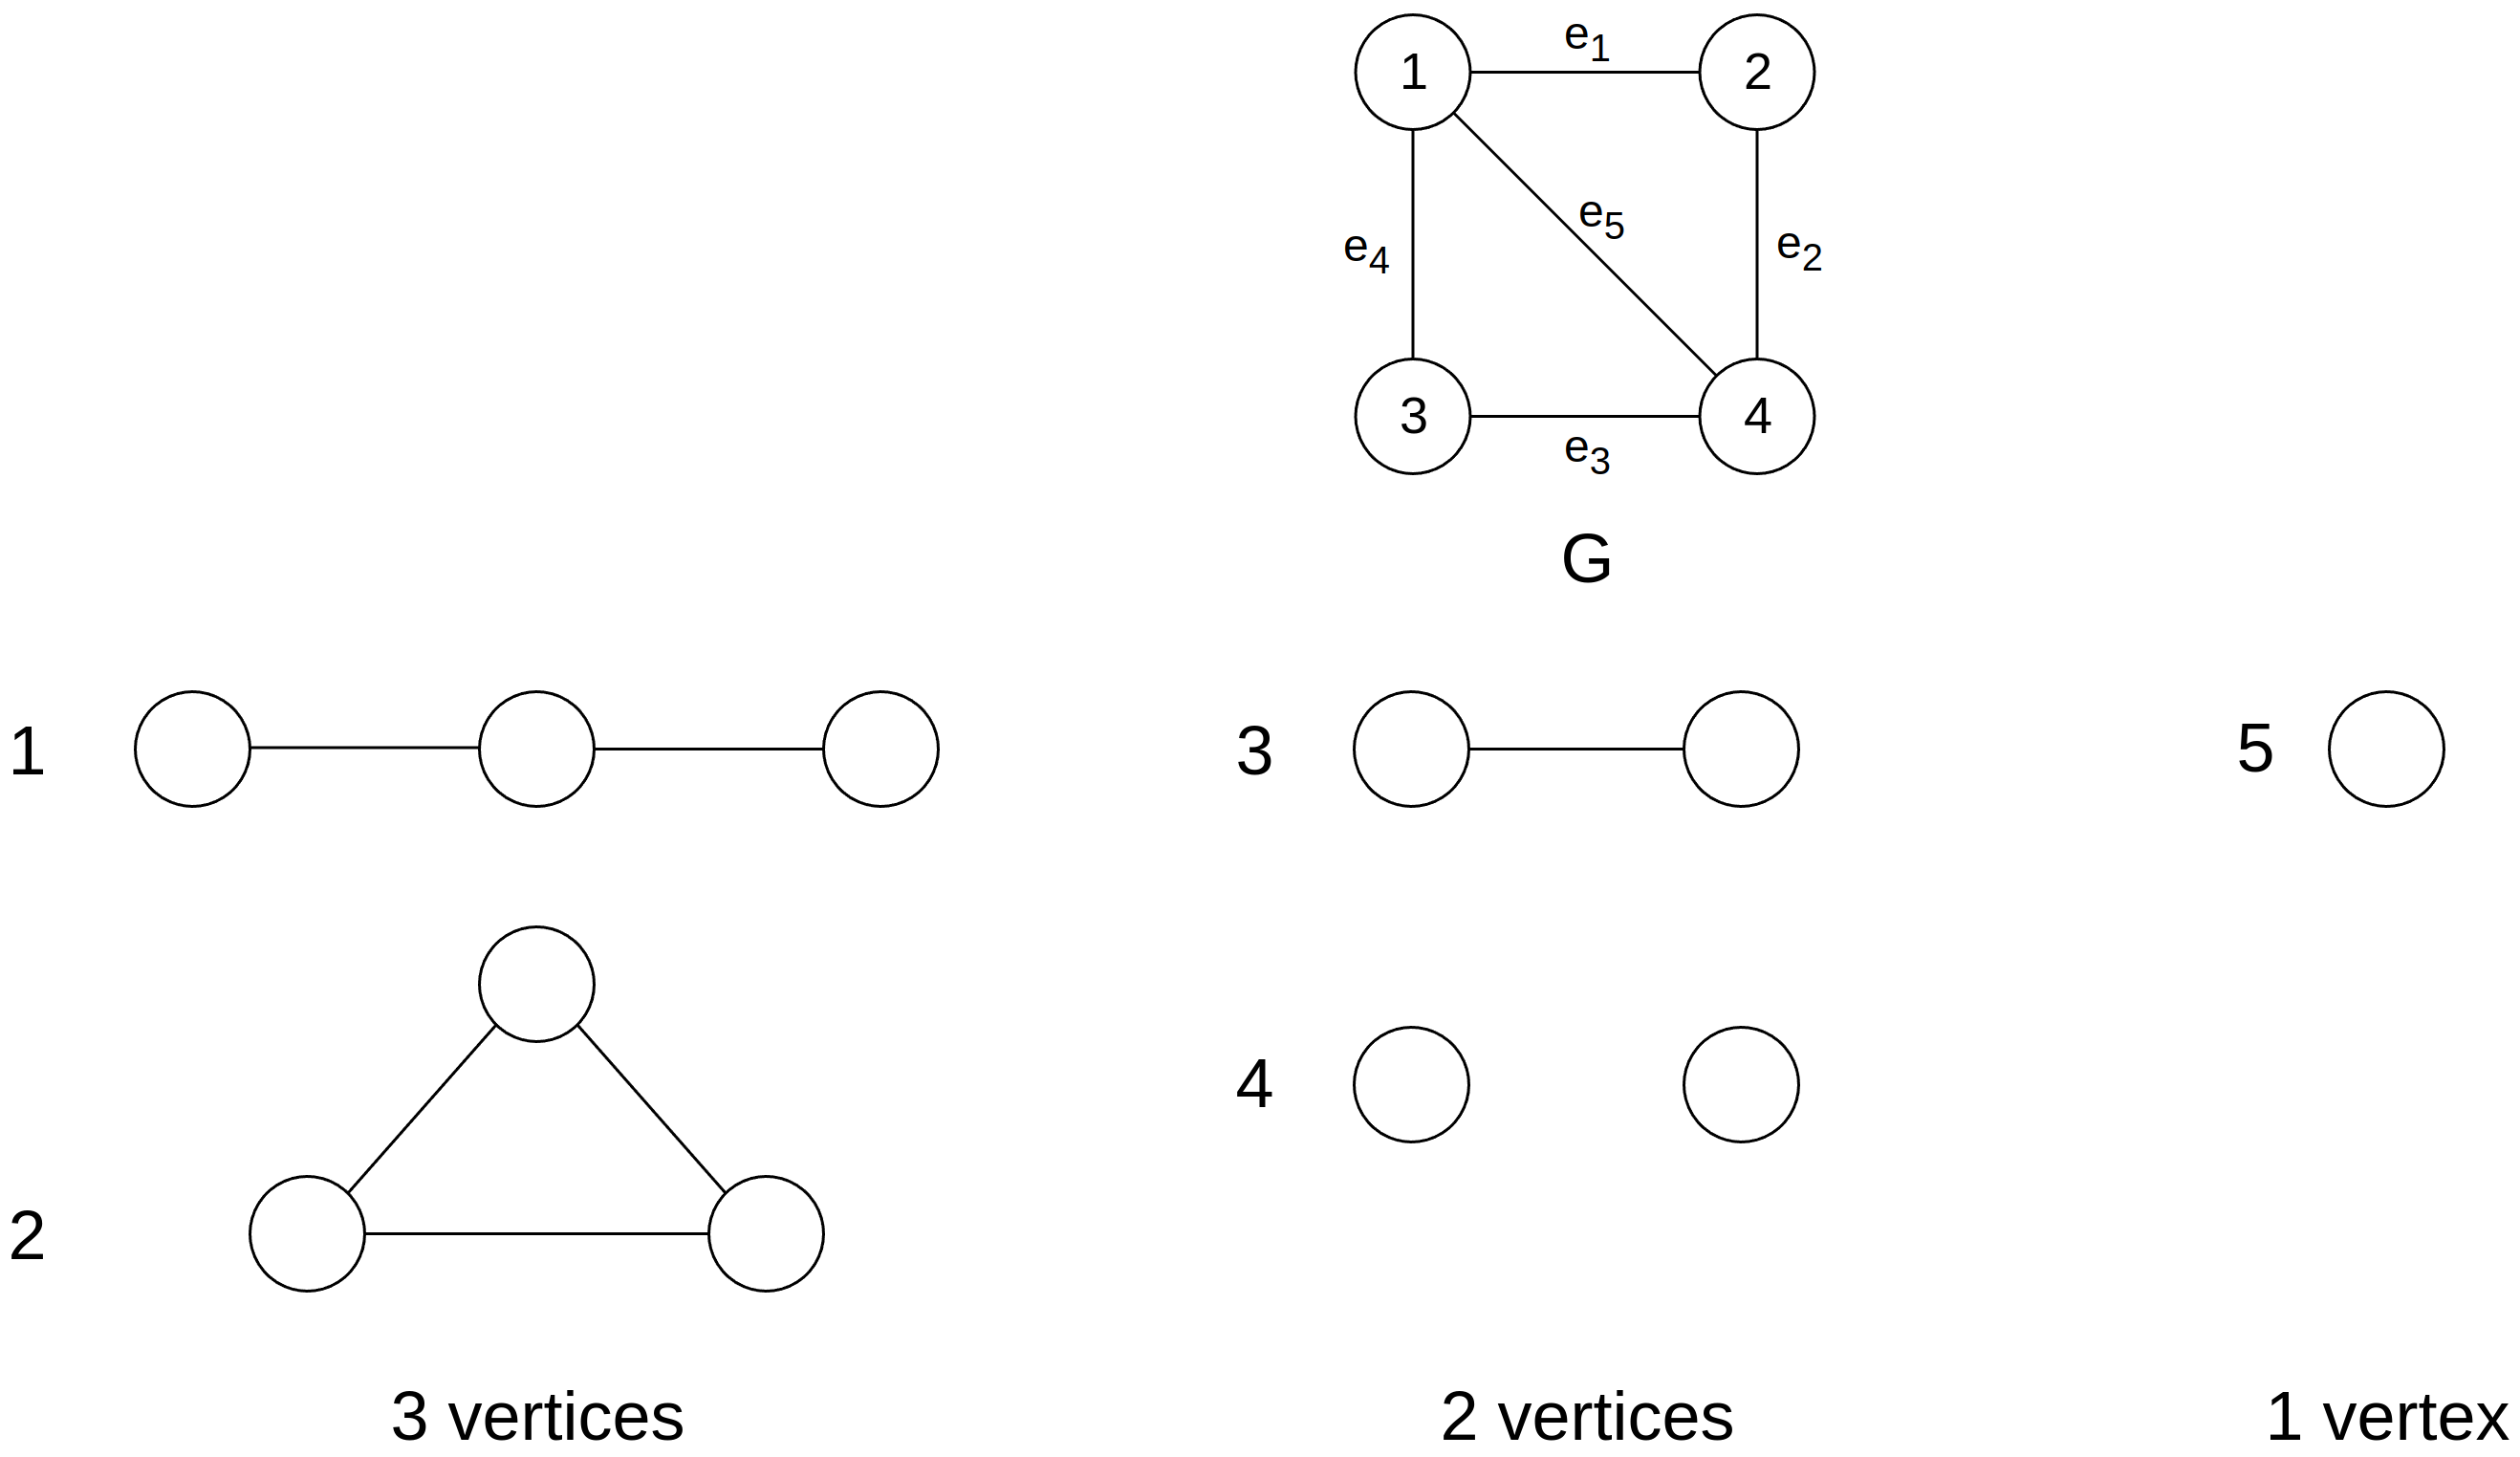
\includegraphics[width=\textwidth,keepaspectratio]{images/induced_subgraphs_example.png}
\caption{A list of all induced subgraphs of a graph G.}
\label{fig:induced_subgraphs}
\end{figure}

For all graphs with $n \ge 2$ vertices, the following statements are always true:

\begin{itemize}
\item there is exactly 1 induced subgraph with $n$ vertices, the original graph itself,
\item there is an induced subgraph with two vertices and either 0 or 1 edges,
\item a single isolated vertex is an induced subgraph,
\item the null graph, a graph with an empty vertex set is also an induced subgraph (while this conflicts with our requirement for a graph to have a non-empty set of vertices, this corresponds to an empty partial permutation, the concept of partial permutations is explained in further detail in Section \ref{sec:semigroups})
\end{itemize}

In Fig. \ref{fig:induced_subgraphs}, we can see all induced subgraphs of a graph $G$ with four vertices. The induced subgraph $S_1$ is a subgraph of G induced by either the set $\{ 2, 3, 4 \}$ or $\{ 1, 2, 3 \}$. The subgraph $S_2$ is an induced subgraph whose vertex set is either $\{ 1, 2, 4\}$ or $\{ 1, 3, 4\}$. Similarly, we can obtain the induced subgraphs $S_3, S_4$ and $S_5$.

We will now explore a relationship that exists between induced subgraphs. The subgraph $S_3$ is obtainable as an induced subgraph from either $S_1$ or $S_2$. The subgraph $S_4$, on the other hand, can be obtained as an induced subgraph only from $S_1$ and not from $S_2$.

Generally, for a graph $G$ with $n$ vertices, every $k$-vertex induced subgraph of $G, k < n$, can be obtained as an induced subgraph from at least one of the induced subgraphs with $k+1$ vertices.

\section{Isomorphism and automorphism of graphs}

\begin{definition}
\label{def:isomorphism}
An isomorphism from a simple graph G to a simple graph H is a bijection: V(G) $\to$ V(H) such that $uv \in E(G)$ if and only if $f(u)f(v) \in E(H)$. We say "G is isomorphic to H", written $G \cong H$ if there is an isomorphism from G to H.
\end{definition}

An example of two isomorphic simple graphs is in Fig. \ref{fig:graph_isomorphism}. The graph $G$ has two vertices with degree 3 ($w$, $z$) and two vertices with degree 2 ($x$, $y$). Both $w$ and $z$ vertices have three neighbors with degrees 3, 2, and 2, and both vertices $x$ and $y$ have two neighbors with degree 3.
In graph $H$, we have two vertices with degree 3 $(c, d)$ and two vertices with degree 2 $(a, b)$. The vertices with degree 3 have neighbors with degrees 3, 2, and 2, and the vertices with degree 2 have two neighbors with degree 3. We can see that while graphs $G$ and $H$ look different visually, they are indeed isomorphic.

More formally, in our example, there exists a function $f$ that maps the vertices of graph $G$ to the vertices of graph $H$ as follows: $f(x) = b$, $f(y) = a$, $f(z) = d$ and $f(w) = c$. The set of edges of graph $H$ is then $E(H) = \{ f(w)f(x), f(w)f(y), f(w)f(z), f(x)f(z), f(y)f(z) \}$.

\begin{figure}[H]
\begin{center}
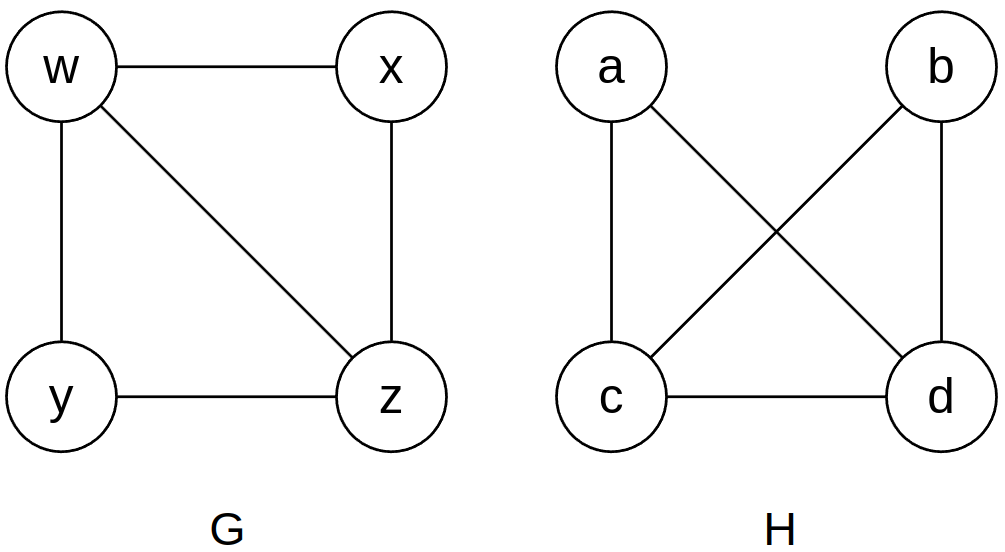
\includegraphics[scale=0.3,keepaspectratio]{images/isomorphism_example.png}
\end{center}
\caption{An example of two isomorphic graphs.}
\label{fig:graph_isomorphism}
\end{figure}

Even though the graphs $G$ and $H$ have the same degree sequence $(3, 3, 2, 2)$, this information alone is insufficient to determine whether the two graphs are isomorphic. Consider the graphs shown in Fig. \ref{fig:non_isomorphism}. Both graphs have the same degree sequence (3, 2, 2, 2, 2, 1, 1, 1), yet they are not isomorphic. The only vertex of degree 3 has neighbors with degrees 2, 1, 1 in one graph but 2, 2, 1 in the other.

We will further examine the adjacency matrix of graph G. An adjacency matrix $A$ is a square matrix in which the value of an element $a_{i, j}$ is 1 if there exists an edge between vertex $i$ and vertex $j$ otherwise it is 0. The adjacency matrix for an undirected graph is symmetric, with simple graphs having only zeroes on the main diagonal.

\begin{figure}[H]
\begin{center}
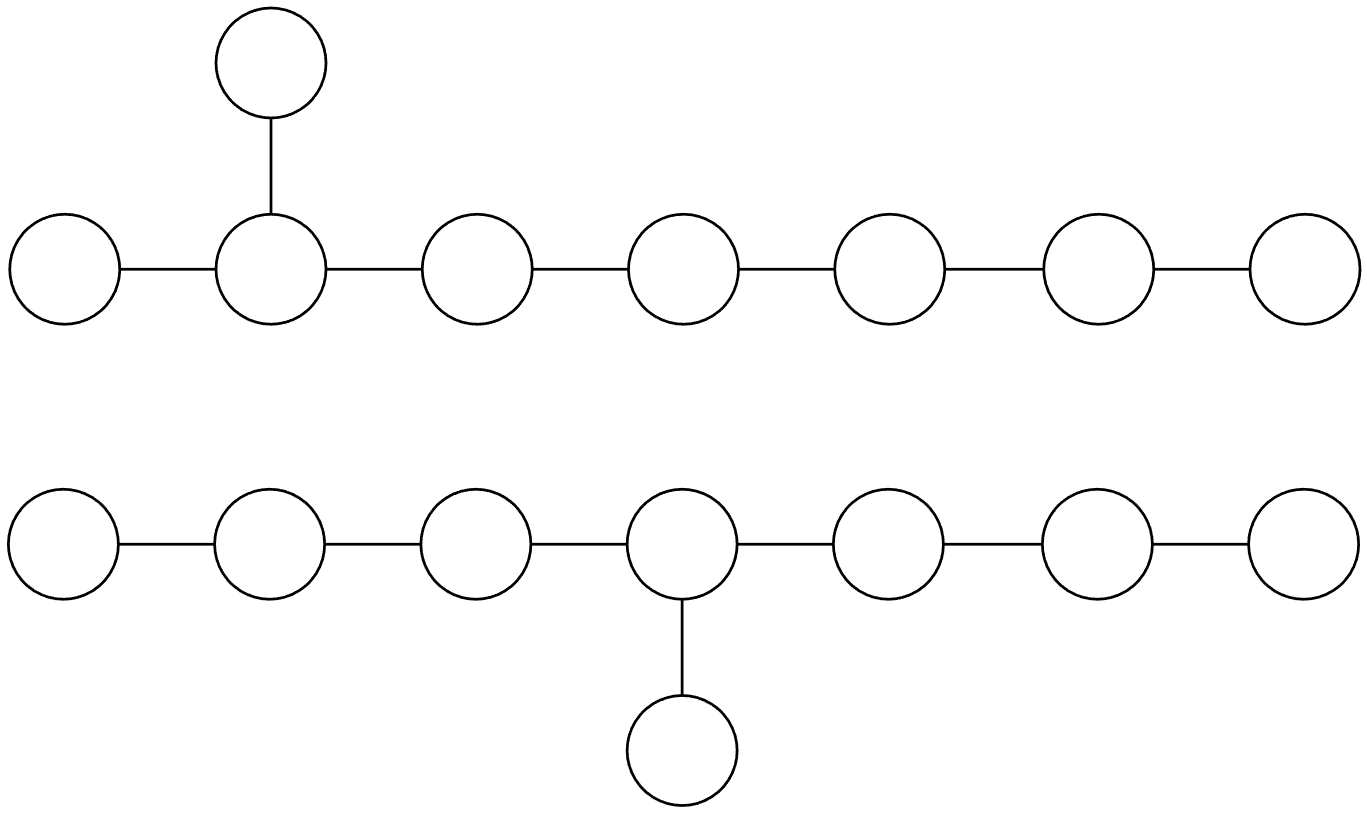
\includegraphics[scale=0.2,keepaspectratio]{images/non_isomorphism_example.png}
\end{center}
\caption{An example of two graphs with the same degree sequence that are not isomorphic.}
\label{fig:non_isomorphism}
\end{figure}

As is stated in Def. \ref{def:isomorphism}, an isomorphism is a bijection that preserves adjacency and non-adjacency. Two graphs $G$ and $H$ are isomorphic if and only if the following holds for their corresponding adjacency matrices $A_G$ and $A_H$:

\begin{equation}
\label{eq:matrices}
A_G = P A_H P^{-1},
\end{equation}
where P is a permutation matrix. A permutation matrix is a square matrix in which there is exactly one element in each row and one element in each column equal to 1, with other elements equal to 0.

Using the aforementioned graphs $G$ and $H$, we get the following matrices, where the matrix $P$ was chosen so that \ref{eq:matrices} holds:

\[
\begin{aligned}
A_G =
\begin{bmatrix}
0&1&1&1\\
1&0&0&1\\
1&0&0&1\\
1&1&1&0
\end{bmatrix}
&
A_H =
\begin{bmatrix}
0&0&1&1\\
0&0&1&1\\
1&1&0&1\\
1&1&1&0
\end{bmatrix}
&
P =
\begin{bmatrix}
0&0&1&0\\
0&1&0&0\\
1&0&0&0\\
0&0&0&1
\end{bmatrix}
\end{aligned}
\]

\begin{definition}
\label{def:isomorphism_class}
An isomorphism class of graphs is an equivalence class of graphs under the isomorphism relation.
\end{definition}

The isomorphism relation is an equivalence relation because it is reflexive, symmetric, and transitive. An equivalence relation partitions a set into equivalence classes, so the isomorphism relation partitions a set of graphs into isomorphism classes. For example, the elements of a set of all triangle graphs (3-cliques) are pairwise isomorphic, so this set forms an isomorphism class.

\begin{definition}
\label{def:automorhism}
An automorphism of G is an isomorphism from G to G.
\end{definition}

\section{Minimal asymmetric graphs}

A graph with only the trivial automorphism group, so its only symmetry is the identity, is called asymmetric. We mention groups in more detail in Section \ref{sec:groups}. Our work aims to examine the 18 finite minimal asymmetric undirected graphs, whose existence was proved by Pascal Schweitzer and Patrick Schweitzer in 2017 \cite{sch17}. Their research confirms the Nešetřil conjecture that there are only finitely many finite minimal asymmetric undirected graphs. The 18 minimal asymmetric graphs are shown in Fig. \ref{fig:minimal_asymmetric}. There are 8 graphs with 6 vertices, 6 graphs with 7 vertices, and 4 graphs with 8 vertices. The information underneath each graph has the form $(v, e, co)$, where $v$ is the number of vertices, $e$ is the number of edges, and $co$ is the complement graph.

\begin{figure}[H]
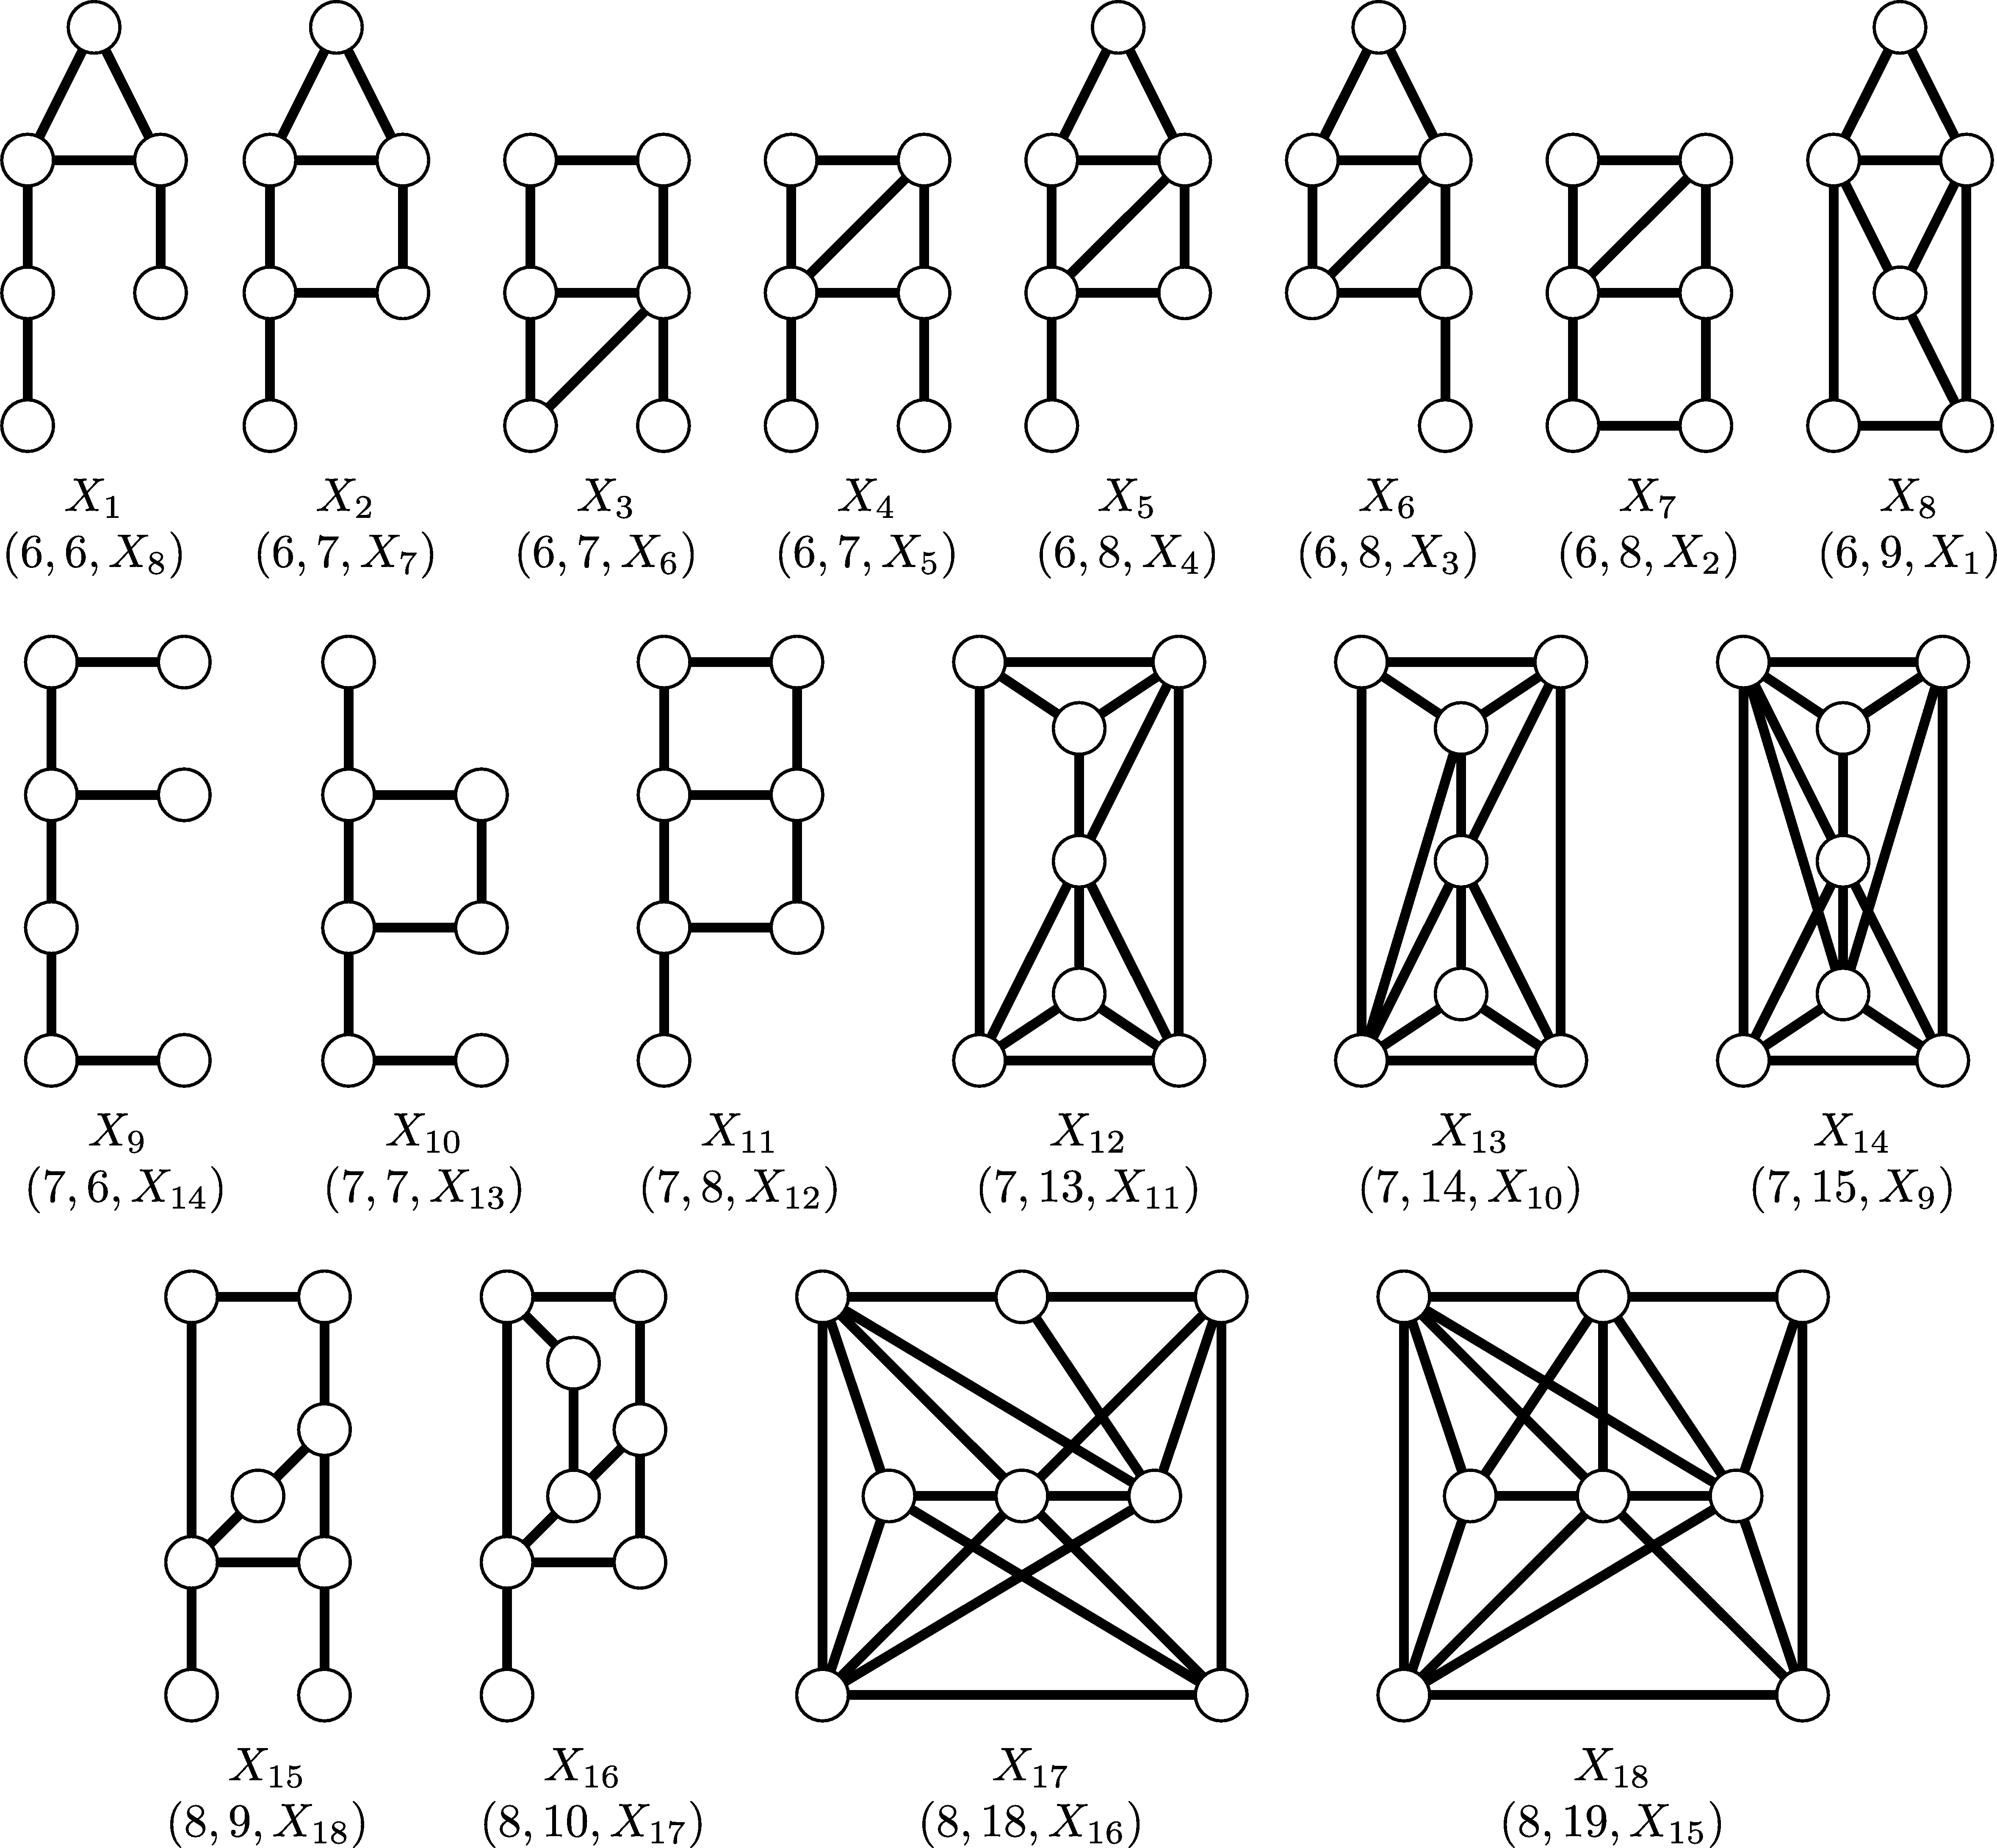
\includegraphics[width=\textwidth,height=\textheight,keepaspectratio]{images/minimal_asymmetric.png}
\caption{A list of all minimal asymmetric graphs \cite{sch17}.}
\label{fig:minimal_asymmetric}
\end{figure}

\section{Group theory}
\label{sec:groups}

In this section, we introduce the necessary terms from group theory and a generalization of groups, the inverse semigroup theory.

Firstly, let's examine the symmetries of a trivial geometric object: a regular pentagon. We can imagine the pentagon as a graph with 5 vertices and 5 edges. We color the vertices using different colors: R (red), G (green), B (blue), Y (yellow), and P (purple). Imagine we fix the pentagon in place, take a copy of it and rotate or flip it so that it precisely covers the original.

\begin{figure}[H]
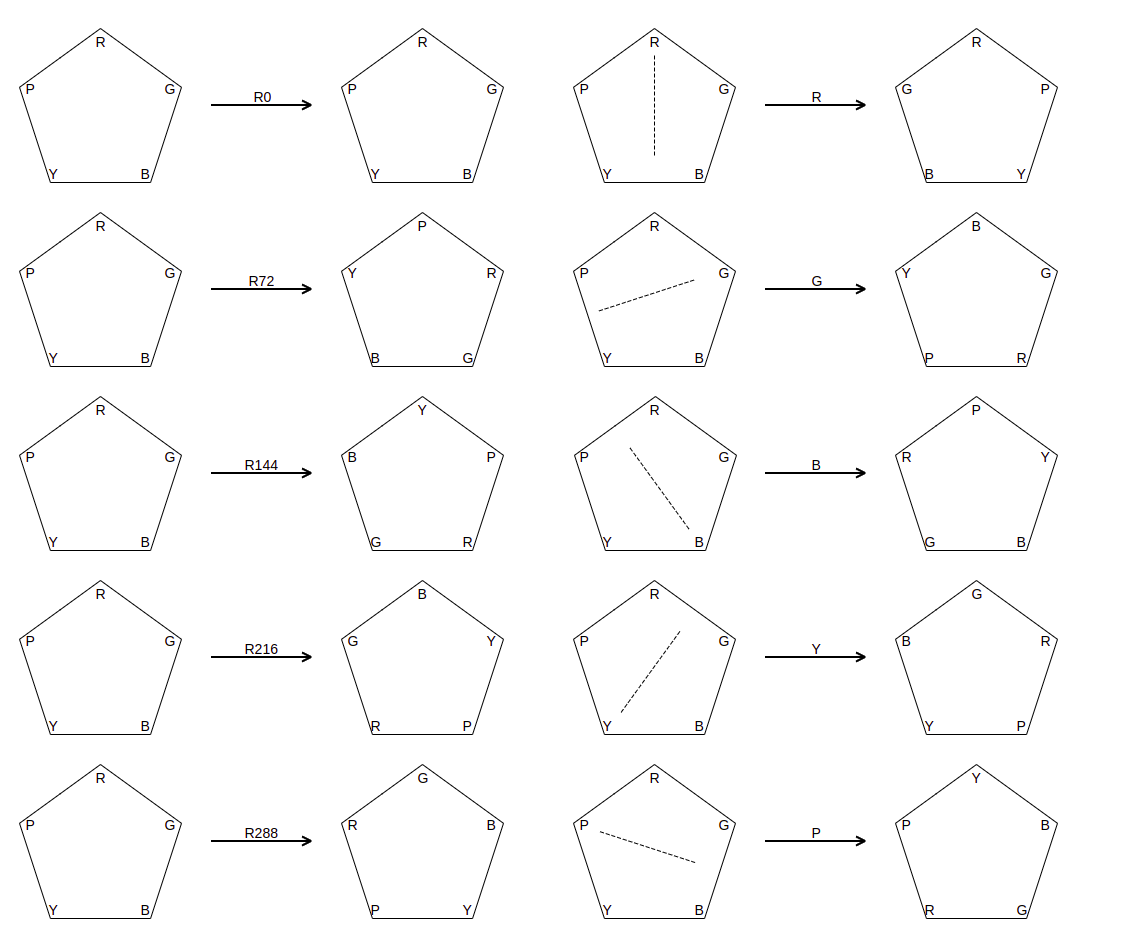
\includegraphics[width=\textwidth,height=\textheight,keepaspectratio]{images/pentagon.png}
\caption{All symmetries of a regular pentagon.}
\label{fig:pentagon_symmetries}
\end{figure}

There are five ways of rotating the pentagon clockwise, by 72, 144, 216, 288, and 360 (same as 0-degree rotation) degrees. We denote these rotations as $RD, D \in \{ 72, 144, 216, 288, 360 \}$. Note that rotations by multiples of these degrees already correspond to one of the 5 rotations listed, so we ignore them. Counter-clockwise rotations correspond to one of the previously mentioned rotations, so we also ignore them.

Next, we can flip the pentagon along the perpendicular bisector of an edge. Altogether, since there are 5 edges in a pentagon, there are 5 such flips possible. We denote these flips as $fC, C \in \{R, G, B, Y, P\}$, to mean flips over the line of symmetry that passes through the $C$-colored vertex.

We can see these 10 symmetries in Fig. \ref{fig:pentagon_symmetries}.

\begin{table}
\small
\begin{tabular}{ c | c c c c c c c c c c }
\hline
* & R0 & R72 & R144 & R216 & R288 & fR & fG & fB & fY & fP \\
\hline
R0 & R0 & R72 & R144 & R216 & R288 & fR & fG & fB & fY & fP \\
R72 & R72 & R144 & R216 & R288 & R0 & fY & fP & fR & fG & fB \\
R144 & R144 & R216 & R288 & R0 & R72 & fG & fB & fY & fP & fR \\
R216 & R216 & R288 & R0 & R72 & R144 & fP & fR & fG & fB & fY \\
R288 & R288 & R0 & R72 & R144 & R216 & fB & fY & fP & fR & fG \\
fR & fR & fY & fG & fP & fB & R0 & R216 & R72 & R288 & R144 \\
fG & fG & fP & fB & fR & fY & R144 & R0 & R216 & R72 & R288 \\
fB & fB & fR & fY & fG & fP & R288 & R144 & R0 & R216 & R72 \\
fY & fY & fG & fP & fB & fR & R72 & R288 & R144 & R0 & R216 \\
fP & fP & fB & fR & fY & fG &R216 & R72 & R288 & R144 & R0 \\
\hline
\end{tabular}
\caption{\label{table:cayley_table} Cayley table for a group of automorphisms of a regular pentagon.}
\end{table}

Let $S$ be the set of all of these symmetries. We can consider all elements of $S$ to be functions that take the original pentagon and map it to itself. Since functions can be composed, we can construct a table in which the element in $i$-th row and $j$-th column is obtained by composing elements $i$ and $j$. This table is called a \emph{Cayley table}, an example of a Cayley table for our set $S$ can be seen in Table \ref{table:cayley_table}.

We can observe that the result of the composition of any two elements from $S$ is also in $S$. This property is called a closure (under function composition). We can also see there exists a unique element $e=R0$ such that $\forall x \in S, xe = ex = x$. This element is called the $identity$. Furthermore, for every element $x \in S$, there exists a single element $y \in S$, such that $xy = yx = e = R0$, and we say that $x$ is the inverse of $y$ (and vice versa). The inverse of an element is unique. This property is also observable in the Cayley table since the identity element $R0$ appears exactly once in each row and each column.

We can conclude that our set $S$ forms a group under function composition (multiplication).

All definitions relating to group theory are taken from \cite{gal12}.

\begin{definition}
\label{def:group}
Let G be a set together with a binary operation (usually called multiplication) that assigns to each ordered pair (a, b) of elements of G an element in G denoted by ab. We say G is a group under this operation if the following properties are satisfied:
\begin{enumerate}
\item \textbf{Associativity} - the operation is associative; that is, (ab)c = a(bc) for all a, b, c in G
\item \textbf{Identity} - there is an element e (called the identity) in G such that ae = ea = a for all a in G
\item \textbf{Inverses} - for each element a in G, there is an element b in G (called an inverse of a) such that ab = ba = e
\end{enumerate}
\end{definition}

\subsection{Permutation groups}

In our above example, we obtained the symmetries of a regular pentagon by permuting its vertices. We showed that the set of all such symmetries forms a group under function composition. This group also forms a permutation group.

\begin{definition}
\label{def:perm}
A permutation of a set A is a function from A to A that is both one-to-one and onto. A permutation group of a set A is a set of permutations of A that forms a group under function composition.
\end{definition}

In other words, a permutation is a bijective function from a set to itself. In total, there are $n!$ different permutations of an $n$-element set. The permutation $\alpha$ can be written in what is known as Cauchy's two-line notation as

\begin{equation}
\alpha =
\begin{pmatrix}
x_1 & x_2 & \cdots & x_n \\
\alpha(x_1) & \alpha(x_2) & \cdots & \alpha(x_n)
\end{pmatrix}
\end{equation}

\subsection{Cycle notation}
\label{sec:cycle_notation}

Cycle notation is an alternative way of representing permutations. For example, let's have a permutation $\alpha$ of the set A = \{1, 2, 3, 4, 5, 6\}, given by $\alpha(1) = 4, \alpha(2) = 3, \alpha(3) = 5, \alpha(4) = 1, \alpha(5) = 2, \alpha(6) = 6$. The permutation $\alpha$ can be written in $cycle$ $notation$ as follows: $\alpha = (14)(523)(6)$. The process of obtaining the cycle notation for a permutation $\alpha$ of a set $A$ is the following:

\begin{enumerate}
\item select any element $x$ from the set $A$
\item successively apply the permutation $\alpha$ to trace all images of element $x$ and write down the results
\item keep repeating the previous step until the successive applications of $\alpha$ trace back to $x$
\item place the results of steps 2-3 inside parentheses so we get a cycle $(x \alpha(x) \\ \alpha(\alpha(x)) \alpha(\alpha(\alpha(x))) ...)$, the element $x$ we started with appears in the cycle only once
\item select an element $y$ not yet in a cycle and repeat the previous steps until all elements of $A$ appear in one of the cycles
\end{enumerate}

We use the term length of a cycle to mean the number of elements in it. Note that the cycles in cycle notation are disjoint (they do not share elements), and we can omit any cycle that fixes an element (a cycle of length 1), so in our previous example, we get $\alpha = (14)(523)$. We will also rewrite the cycles so that the minimal element of each cycle is listed first: $\alpha = (14)(235)$.

\subsection{Orbits and stabilizers}

\begin{definition}
Let $G$ be a group of permutations of a set $S$. For each $s$ in $S$, let $orb_G(s) = \{\phi(s) | \phi \in G \}$. The set $orb_G(s)$ is a subset of $S$ called the orbit of $s$ under $G$. We use $|orb_G(s)|$ to denote the number of elements in $orb_G(s)$.
\end{definition}

\begin{definition}
Let G be a group of permutations of a set S. For each i in S, let $stab_G(i) = \{ \phi \in G | \phi(i) = i \}$. We call $stab_G(i)$ the stabilizer of i in G.
\end{definition}

\begin{definition}
\label{def:group_order}
Let G be a finite group of permutations of a set S. Then, for any i from S, $|G| = |orb_G(i)| |stab_G(i)|$.
\end{definition}

Let's examine the graph $G$, $V(G) = \{1, 2, 3, 4, 5, 6\}$ shown in Fig. $\ref{fig:cycle_notation_graph}$. The group of automorphisms of $G$ is $Aut(G) = \{ (1)(2)(3)(4)(5)(6), (1)(23)(45)(6),$ $(16)(24)(35), (16)(25)(34) \}$. The orbit of an element $x$ are all vertices to which $x$ gets mapped by some automorphism in the automorphism group $Aut(G)$. For example, the orbits of vertex $1$ are $\{ 1, 6 \}$ and the orbits of vertex $2$ are $\{ 2, 3, 4, 5 \}$.

The stabilizers of an element $x$ are those elements of $Aut(G)$, that map $x$ to itself (stabilize it in its place). In other words, we can easily find the stabilizers of $x$ by finding all elements of $Aut(G)$, in which the length of a cycle containing $x$ is 1. The stabilizers of $1$ are $\{ (1)(2)(3)(4)(5)(6), (1)(23)(45)(6) \}$ and the stailizer of $2$ is $\{(1)(2)(3)(4)(5)(6)\}$.

\begin{figure}[H]
\begin{center}
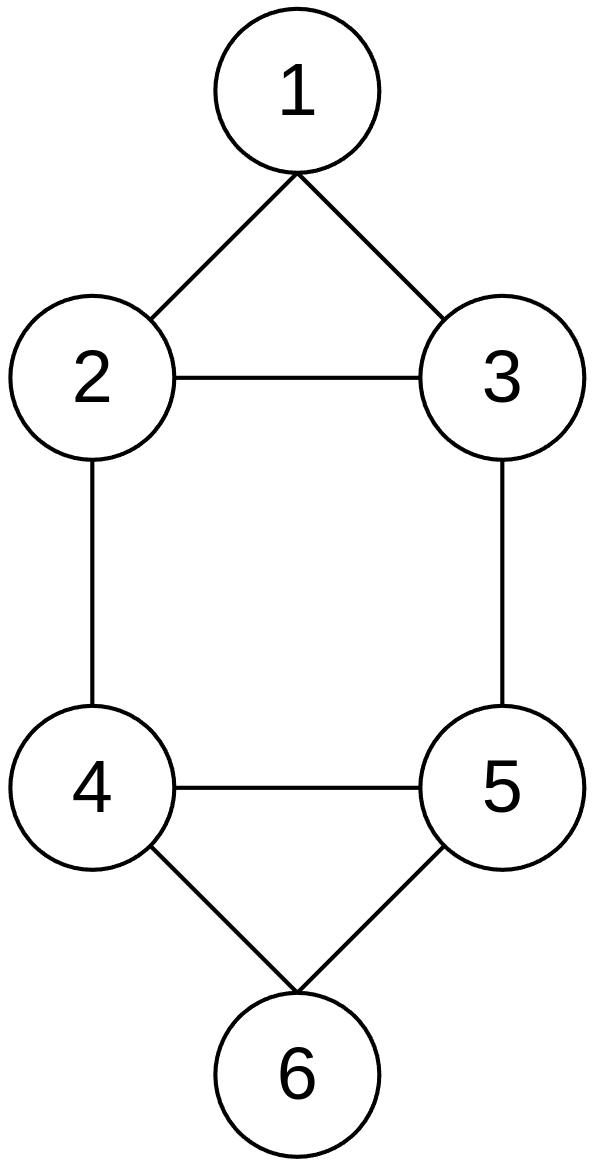
\includegraphics[scale=0.2,keepaspectratio]{images/cycle_notation_graph.png}
\end{center}
\caption{Graph G with 4 automorphisms.}
\label{fig:cycle_notation_graph}
\end{figure}

The Definition $\ref{def:group_order}$, known as the $orbit-stabilizer$ $theorem$, also holds as $|G| = 4 = |orb_G(1)| |stab_G(1)| = |orb_G(2)| |stab_G(2)|$.

\section{Semigroups}
\label{sec:semigroups}

We now explore the concept of inverse semigroups, a generalization of groups. A semigroup is a set with an associative binary operation that does not need to have all of the properties groups have. For this reason, every group is also a semigroup, but not every semigroup satisfies the properties necessary to be a group. Definitions in this section are taken from the book \cite{law98}.

\begin{definition}
\label{semigroup_def}
A non-empty set together with an associative multiplication is called a semigroup, and a semigroup admitting an identity (neutral) element is called a monoid. A monoid S is said to be an inverse monoid if, for every $s \in S$, there exists a unique element $s^{-1} \in S$, called the inverse of s, such that $s s^{-1} s=s$ and $s^{-1} s s^{-1} = s^{-1}$ hold. Note that the operation of taking inverses has the properties that $(s^{-1})^{-1} = s$ and $(st)^{-1} = t^{-1} s^{-1}$ for any $s, t \in S$.
\end{definition}

\subsection{Partial permutations}
\label{sec:partial_permutation}

We introduce the concept of partial permutations and describe a modification of the cycle notation we use to represent them.

\begin{definition}
\label{def:partial_perm}
The set of all bijections between subsets of a set X, including the empty set is called the set of partial permutations of X and is denoted PSym(X). If $\psi : Y \to Z \in PSym(X), Y, Z \subseteq X$, then Y and Z are the domain (denoted dom) and range (ran) of $\psi$, respectively.
\end{definition}

To store partial permutations in an easy-to-understand format we modify the cycle notation described in Section \ref{sec:cycle_notation}. Cycle notation is insufficient for partial permutations, since there might be elements that appear in the domain but not in the range, in which case we cannot cyclically permute them. In cases when the process of obtaining a cycle as described in Section \ref{sec:cycle_notation} ends outside the domain, we use a $path$ notation instead \cite{jjss21}. A path is denoted as $[x_k, \cdots , x_2, x_1)$, where all elements are distict and $k \ge 2$. We read a path notation from right to left, so for example a path $[5312)$ denotes a partial permutation that maps 2 to 1, 1 to 3, 3 to 5, and 5 does not get mapped to anything, it is undefined.

\subsection{Green's relations}

Definitions and concepts described in this section are from \cite[Section~3.3]{jjss21} and \cite[Section~3]{jaj22}.

\begin{definition}
\label{green_rel_def}
Let S be an arbitrary monoid and $a, b \in S$ be arbitrary elements. We define two equivalence relations $\mathcal{L}$ and $\mathcal{R}$ the following way:
\begin{enumerate}
\item a $\mathcal{L}$ b if and only if there exist $x, y \in S$ such that xa = b and yb = s.
\item a $\mathcal{R}$ b if and only if there exist $x, y \in S$ such that ax = b and by = a.
\end{enumerate}
\end{definition}

Applying the general definition of Green's relations on partial permutations, we get that the $\mathcal{R}$ relations coincide with partial permutations sharing the same range, and the $\mathcal{L}$ relations coincide with partial permutations sharing the same domain.

\begin{figure}[H]
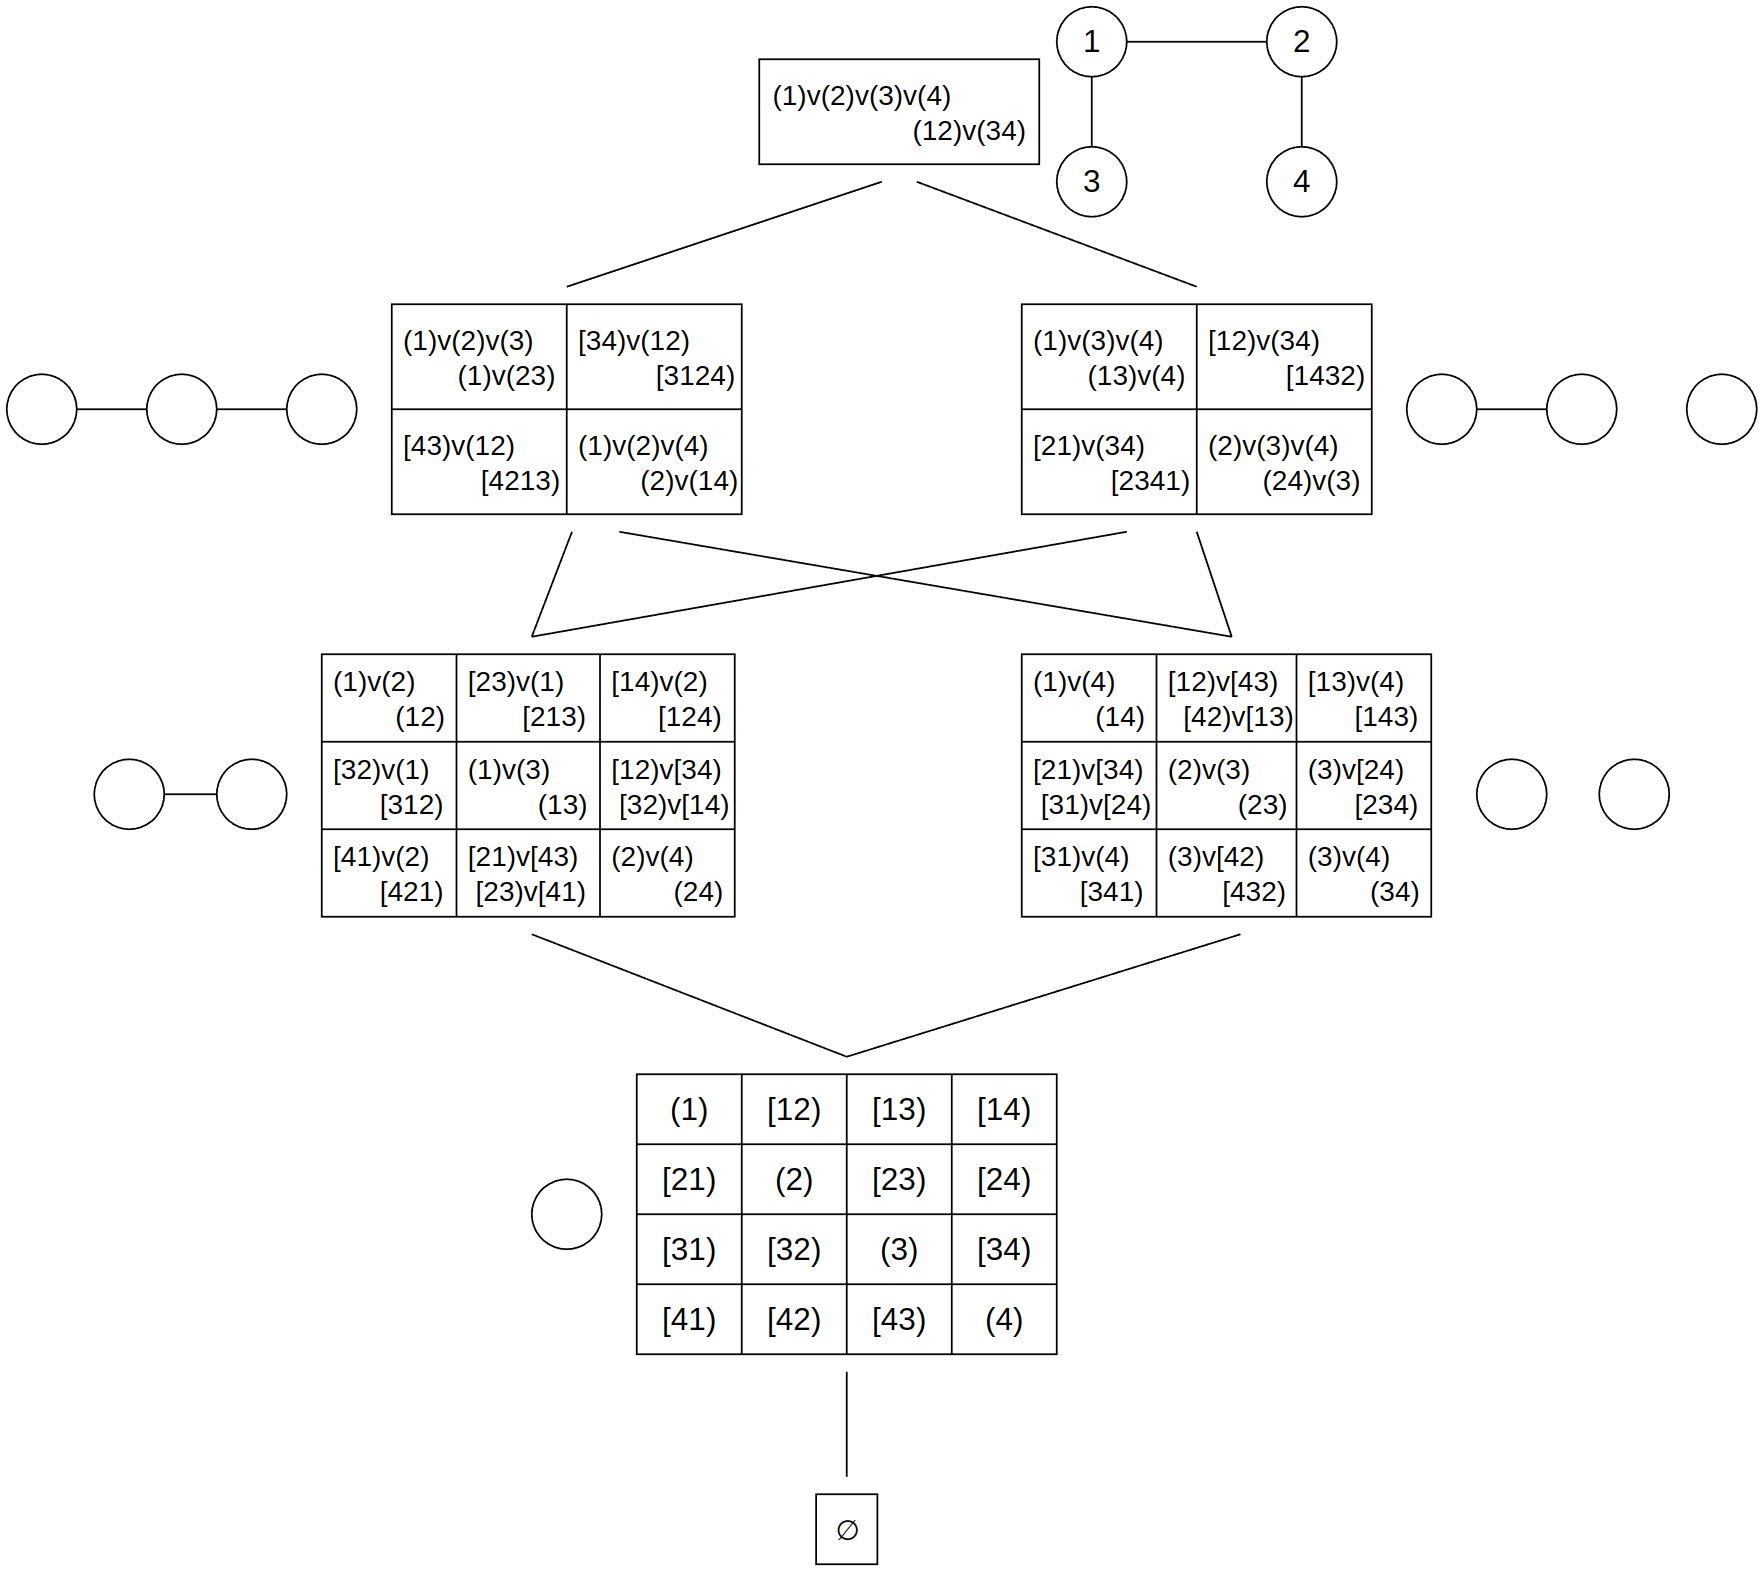
\includegraphics[width=\textwidth,height=\textheight,keepaspectratio]{images/partial_sym_example.png}
\caption{An example of a partial automorphism monoid of a graph with 4 vertices}
\label{fig:partial_sym_example}
\end{figure}

We define a third Green's equivalence relation as $\mathcal{H} = \mathcal{R} \cap \mathcal{L}$. In an inverse monoid, every $\mathcal{R}$-class and $\mathcal{L}$-class contain exactly one idempotent, and $\mathcal{H}$-classes that contain them are the maximal subgroups of the inverse monoid.

The last Green's equivalence relation we need to define contains both $\mathcal{R}$ and $\mathcal{L}$ relations as is defined as $\mathcal{D} = \mathcal{R} \circ \mathcal{L} = \mathcal{L} \circ \mathcal{R}$, where $\circ$ is the composition of relations. In the partial automorphism monoid of graph $G$, the $\mathcal{D}$-classes correspond to the isomorphism classes of vertex-induced subgraphs of $G$.

Fig. \ref{fig:partial_sym_example} shows the partial automorphism monoid of a graph $G$ with 4 vertices. In the visual representation of a monoid, we have "levels" where each level contains $\mathcal{D}$-classes of induced subgraphs with the same number of vertices. At the top is an induced subgraph with 4 vertices, the graph $G$ itself. Below it, in the second level, we have all isomorphism classes corresponding to subgraphs with 3 vertices. Generally, for a graph with $n$ vertices, the partial automorphism monoid consists of $n+1$ levels. At the bottom of every partial automorphism monoid, we have a $\mathcal{D}$-class containing $\emptyset$, which corresponds to a map with an empty domain.

Let's further examine the $\mathcal{D}$-class of an induced subgraph with 2 vertices and 1 edge. As mentioned earlier, the $\mathcal{R}$ relation coincides with partial permutations that share the same range. In the $\mathcal{D}$-class, visually represented as what is known as an "eggbox" diagram, partial permutations belonging to the same $\mathcal{R}$-class are in the same row. The first row in our example contains the following partial permutations: $\{ (1)v(2), (12), [23)v(1), [213), [14)v(2), [124) \}$, that share the same range $\{1, 2\}$. The elements in the second row share the range $\{ 1, 3\}$, and in the last row we have the range $\{ 2, 4 \}$.

Similarly, partial permutations that share the same domain belong to the same $\mathcal{L}$-class and are in the same column. All partial permutations in the $\mathcal{L}$-class $\{ (1)v(2), (12), [32)v(1), [312), [41)v(2), [421) \}$ share the same domain $\{ 1, 2\}$ and all these elements are in the first column. The second column contains elements with domain $\{ 1, 3 \}$ and elements with domain $\{ 2, 4 \}$ are in the last column.

When constructing the $\mathcal{D}$-class, we arrange $\mathcal{R}$-classes and $\mathcal{L}$-classes so that $\mathcal{H}$-classes containing idempotents are on the main diagonal. These $\mathcal{H}$-classes containing idempotents form a group.